\section{Definición de relaciones}

\subsection{¿Qué es una relación?}


En matemáticas, una de las formas más naturales de establecer conexiones entre elementos de distintos conjuntos es a través de las relaciones.

En ciencias de la computación, las relaciones juegan un rol fundamental en múltiples contextos. Permiten modelar datos y sus vínculos, como en bases de datos relacionales; representan estructuras como grafos en algoritmos y redes; y son esenciales para describir transiciones de estado, dependencias, ordenamientos y equivalencias. Comprender las propiedades de las relaciones permite, por ejemplo, optimizar consultas en SQL, verificar invariantes en programas o formalizar sistemas lógicos complejos.


\begin{definitionblock}{Relación binaria}
Una \textbf{relación binaria} entre dos conjuntos $A$ y $B$ es un \textbf{subconjunto del producto cartesiano} $A \times B$. Es decir, es un conjunto de pares ordenados $(a,b)$ donde $a \in A$ y $b \in B$.
\end{definitionblock}

\paragraph{Notación.} Si $R \subseteq A \times B$, entonces decimos que los elementos $a_0 \in A$ y $b_0 \in B$ están relacionados por $R$ si $(a_0, b_0) \in R$. Esto lo denotamos como:
\[ a_0 \, R \, b_0. \]
Si no están relacionados, usamos:
\[ a_0 \, \centernot R \, b_0 \quad \text{ o } \quad (a_0, b_0) \notin R. \]

\subsubsection*{Ejemplo: Relación de divisibilidad.} Consideremos los conjuntos $\mathbb{N}$ (naturales) y $\mathbb{N}_0$ (naturales con cero). Podemos definir la relación de divisibilidad como:
\[
\mid \,=\, \{ (a, k \cdot a) \mid a \in \mathbb{N},~k \in \mathbb{N}_0 \}.
\]
Otra forma equivalente de definirla:
\[
a \mid b \quad \Leftrightarrow \quad \exists k \in \mathbb{N}_0 \text{ tal que } b = k \cdot a.
\]

\subsubsection*{Ejemplo: Base de datos relacional.} 
En una base de datos relacional, una relación puede modelar la asignación de estudiantes a cursos como un subconjunto del producto cartesiano entre el conjunto de estudiantes $E$ y el conjunto de cursos $C$. Por ejemplo, si $(e, c) \in R$ indica que el estudiante $e$ está inscrito en el curso $c$.
% $R \subseteq E \times C$ es una relación que puede analizarse para detectar redundancias, restricciones de integridad o prerequisitos utilizando propiedades como la transitividad o la unicidad.


\subsection{Representación de relaciones}
Cuando los conjuntos involucrados son finitos, podemos representar gráficamente una relación como un grafo dirigido. Una flecha desde $a \in A$ hacia $b \in B$ indica que $a \, R \, b$.


\begin{figure}[h]
\centering
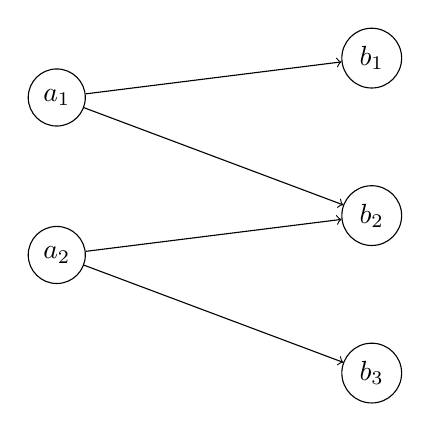
\begin{tikzpicture}[every node/.style={circle,draw}, node distance=2cm]
  \node (a1) at (0,2) {$a_1$};
  \node (a2) at (0,0) {$a_2$};
  \node (b1) at (4,2.5) {$b_1$};
  \node (b2) at (4,0.5) {$b_2$};
  \node (b3) at (4,-1.5) {$b_3$};

  \draw[->] (a1) -- (b1);
  \draw[->] (a1) -- (b2);
  \draw[->] (a2) -- (b2);
  \draw[->] (a2) -- (b3);
\end{tikzpicture}
\caption{En esta ilustración, los nodos del lado izquierdo representan elementos de un conjunto $A$, los del lado derecho a un conjunto $B$, y las flechas indican los pares relacionados en $R \subseteq A \times B$.}
\end{figure}



\subsubsection*{¿Cuántas relaciones existen entre dos conjuntos finitos $A$ y $B$? }
Si $A$ tiene $m$ elementos y $B$ tiene $n$, entonces el conjunto $A \times B$ tiene $m \cdot n$ elementos. Por lo tanto, existen $2^{mn}$ relaciones distintas entre $A$ y $B$.

Esto muestro cómo una definición tan simple como ``subconjunto del producto cartesiano'' puede esconder una riqueza combinatoria enorme. Incluso con conjuntos pequeños, la cantidad de posibles relaciones crece exponencialmente. Esto tiene consecuencias profundas en ciencias de la computación. Por ejemplo,  en \textbf{bases de datos}, cada relación representa una tabla posible; entender su espacio total ayuda a evaluar restricciones, integridad referencial y optimización.
  



\subsection{Relaciones sobre un conjunto}

En el caso particular en que una relación $R$ relaciona elementos de un conjunto consigo mismo, es decir, $R \subseteq A \times A$, decimos que $R$ es una \textbf{relación sobre el conjunto $A$}.

\paragraph{Ejemplos.}
\begin{itemize}
  \item $R = \{(a,b) \mid a \leq b\}$ sobre $\mathbb{N}$.
  \item $R = \{(a,b) \mid a + b \leq 3\}$ también sobre $\mathbb{N}$.
\end{itemize}

\subsection{Propiedades de las relaciones}

Al estudiar relaciones sobre un conjunto $A$, es común interesarse por ciertas propiedades estructurales que éstas pueden tener. 
De hecho, cada una de estas propiedades ya las expresamos usando lógica de predicados. 


\begin{definitionblock}{Propiedades fundamentales}
Sea $R \subseteq A \times A$ una relación sobre $A$. Decimos que:
\begin{itemize}
  \item $R$ es \textbf{reflexiva} si $(a,a) \in R$ para todo $a \in A$.
  \item $R$ es \textbf{simétrica} si $(a,b) \in R$ implica $(b,a) \in R$.
  \item $R$ es \textbf{antisimétrica} si $(a,b) \in R$ y $(b,a) \in R$ implica $a = b$.
  \item $R$ es \textbf{transitiva} si $(a,b) \in R$ y $(b,c) \in R$ implica $(a,c) \in R$.
\end{itemize}
\end{definitionblock}



% \paragraph{Ejercicio.} ¿Qué propiedades cumple la relación vacía $R = \emptyset$?

\paragraph{Ejemplo:} Sobre el conjunto de enteros $\mathbb{Z}$:
\begin{itemize}
  \item $R_1 = \{(a,b) \mid a \leq b\}$ es reflexiva, antisimétrica y transitiva.
  \item $R_2 = \{(a,b) \mid a \mid b\}$ también cumple las tres propiedades anteriores.
  \item $R_3 = \{(a,b) \mid a + b \leq 3\}$ es simétrica, pero no transitiva ni reflexiva.
\end{itemize}

\section{Relaciones de orden}
Las relaciones de orden nos permiten capturar de manera formal la noción de jerarquía, precedencia o comparación entre elementos. Son fundamentales para modelar estructuras como cronogramas de tareas, jerarquías de clases, árboles de decisión, relaciones de dependencia en grafos y muchas otras situaciones donde ciertos elementos están "por encima" o "antes" que otros. 


\begin{definitionblock}{Relaciones de orden}
Una relación $R \subseteq A \times A$ se llama:
\begin{itemize}
  \item \textbf{Orden parcial} si es reflexiva, antisimétrica y transitiva.
  \item \textbf{Orden total} si además, para todo $a,b \in A$, se cumple que $(a,b) \in R$ o $(b,a) \in R$.
\end{itemize}
\end{definitionblock}

\paragraph{Ejemplo.}
\begin{itemize}
  \item La relación $\leq$ sobre $\mathbb{N}$ es un orden total.
  \item La inclusión $\subseteq$ sobre $2^S$ es un orden parcial, pero no total si $S \neq \emptyset$.
\end{itemize}



\section{Relaciones de equivalencia}
Las relaciones de equivalencia permiten formalizar la idea de que dos elementos son esencialmente ``lo mismo'' bajo cierto criterio. Estas relaciones son centrales para definir particiones de conjuntos, clases de objetos indistinguibles y estructuras algebraicas como clases de congruencia, espacios cociente o tipos abstractos de datos.

En ciencias de la computación, se usan para identificar elementos equivalentes en optimización de código, hashing, agrupamiento de datos y en la definición de semánticas de programas (por ejemplo, dos expresiones que se evalúan igual en todo contexto son consideradas equivalentes).


\begin{definitionblock}{Relación de equivalencia}
Una relación $R$ sobre un conjunto $A$ es una \textbf{relación de equivalencia} si es reflexiva, simétrica y transitiva.
\end{definitionblock}

\paragraph{Ejemplo: congruencia módulo $p$.} Para $p \geq 2$ y $a,b \in \mathbb{Z}$,
\[
a \equiv_p b \quad \Leftrightarrow \quad p \mid (a - b)
\]
es una relación de equivalencia.

% \paragraph{Ejercicio.} Demuestre que si $R$ es simétrica y transitiva, y para cada $a \in A$ existe $b$ tal que $(a,b) \in R$, entonces $R$ es reflexiva y por ende, una relación de equivalencia.




\bigskip
\begin{table}[h]
\centering
\resizebox{\textwidth}{!}{%
\begin{tabular}{|l|c|c|c|c|l|}
\hline
\textbf{Tipo de relación} & \textbf{Reflexiva} & \textbf{Simétrica} & \textbf{Antisimétrica} & \textbf{Transitiva} & \textbf{Ejemplo} \\
\hline
Relación de equivalencia & \checkmark & \checkmark & -- & \checkmark & Congruencia módulo $n$ \\
Orden parcial & \checkmark & -- & \checkmark & \checkmark & $\subseteq$, $\leq$ en $\mathbb{N}$ \\
Orden total & \checkmark & -- & \checkmark & \checkmark & $\leq$ en $\mathbb{Z}$ \\
\hline
\end{tabular}
}
\caption{Relación entre propiedades y tipos de relaciones comunes}
\end{table}

\subsection{Clases de equivalencia}
Una de las consecuencias más interesantes de tener una relación de equivalencia es que nos permite agrupar los elementos del conjunto en subconjuntos disjuntos llamados \textbf{clases de equivalencia}. Cada clase está formada por todos los elementos que son equivalentes entre sí respecto a la relación $R$. Esta idea permite clasificar elementos según algún criterio de equivalencia y es muy útil tanto en matemáticas como en ciencias de la computación, por ejemplo, al agrupar datos, detectar redundancias o definir estados equivalentes en autómatas.


\begin{definitionblock}{Clase de equivalencia}
Dada una relación de equivalencia $R$ sobre un conjunto $A$ y un elemento $a \in A$, la \textbf{clase de equivalencia} de $a$, denotada $[a]_R$, es:
\[
[a]_R = \{ b \in A \mid (a,b) \in R \}
\]
\end{definitionblock}

\paragraph{Ejemplo: módulo 3.}
\begin{align*}
[0]_{\equiv_3} &= \{ ..., -6, -3, 0, 3, 6, ... \} \\
[1]_{\equiv_3} &= \{ ..., -5, -2, 1, 4, 7, ... \} \\
[2]_{\equiv_3} &= \{ ..., -4, -1, 2, 5, 8, ... \}
\end{align*}

\begin{thmblock}{Lema: Caracterizaciones de equivalencia}  Si $R$ es una relación de equivalencia sobre $A$, entonces para cualquier $a, b \in A$ se cumple:
\[
(a,b) \in R \quad \Leftrightarrow \quad [a]_R = [b]_R \quad \Leftrightarrow \quad [a]_R \cap [b]_R \neq \emptyset
\]
\end{thmblock}
\begin{proof}
Demostremos las implicaciones una por una:

\begin{itemize}
  \item[$(1 \Rightarrow 2)$] Supongamos que $(a,b) \in R$. Queremos probar que $[a]_R = [b]_R$.\
  Sea $x \in [a]_R$, es decir, $(a,x) \in R$. Como $(a,b) \in R$ y $R$ es simétrica y transitiva, se sigue que $(b,x) \in R$, por lo tanto $x \in [b]_R$, y así $[a]_R \subseteq [b]_R$.\
  Análogamente, $(b,a) \in R$ (por simetría), y el mismo argumento muestra que $[b]_R \subseteq [a]_R$. Entonces $[a]_R = [b]_R$.

  \item[$(2 \Rightarrow 3)$] Supongamos que $[a]_R = [b]_R$. Entonces tienen al menos un elemento en común (por ejemplo $a \in [a]_R$), por lo tanto $[a]_R \cap [b]_R \neq \emptyset$.

  \item[$(3 \Rightarrow 1)$] Supongamos que $[a]_R \cap [b]_R \neq \emptyset$. Entonces existe $x \in A$ tal que $(a,x) \in R$ y $(b,x) \in R$. Como $R$ es simétrica, $(x,b) \in R$ y luego por transitividad, $(a,b) \in R$.
\end{itemize}
Por lo tanto, todas las implicaciones se cumplen y las tres condiciones son equivalentes.
\end{proof}


\section{Relaciones de equivalencia y particiones}

Vimos cómo una relación de equivalencia nos permite agrupar los elementos de un conjunto en clases de equivalencia, donde todos los elementos de una clase están relacionados entre sí. Esta estructura naturalmente nos lleva a la noción de \textbf{partición}, que es una forma de dividir un conjunto en subconjuntos que no se superponen y que cubren completamente al conjunto original.

Las clases de equivalencia inducidas por una relación de equivalencia forman una partición del conjunto. 
Inversamente, toda partición de un conjunto define una relación de equivalencia entre elementos. 
% Esta correspondencia entre relaciones de equivalencia y particiones es una idea fundamental que aparece en múltiples áreas de la matemática y la computación, desde estructuras algebraicas hasta clasificación de datos o estados equivalentes en autómatas.

\bigskip
\begin{definitionblock}{Partición}
Una \textbf{partición} de un conjunto $A$ es una colección de subconjuntos no vacíos, disjuntos dos a dos, cuya unión es $A$.
\end{definitionblock}

\begin{figure}[h]
\begin{center}
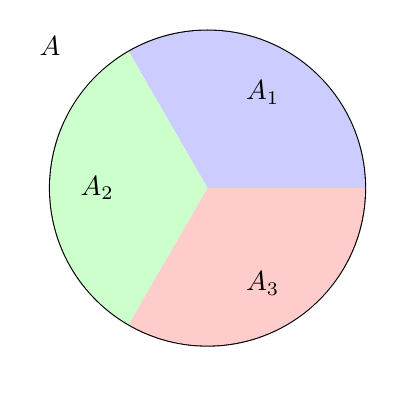
\begin{tikzpicture}[scale=1]
  \def\r{2}
  % Dibujamos el círculo completo
  \draw[thick] (0,0) circle (\r);

  % Llenamos los 3 sectores, cada uno cubriendo 120° del círculo
  \fill[blue!20] (0,0) -- (0:\r) arc (0:120:\r) -- cycle;
  \fill[green!20] (0,0) -- (120:\r) arc (120:240:\r) -- cycle;
  \fill[red!20] (0,0) -- (240:\r) arc (240:360:\r) -- cycle;

  % Etiquetamos cada sector
  \node at (60:1.4) {$A_1$};
  \node at (180:1.4) {$A_2$};
  \node at (300:1.4) {$A_3$};
  \node at (-2,1.8) {\bm{$A$}};
\end{tikzpicture}
\end{center}
\caption{En esta ilustración, el conjunto $A$ está dividido en tres subconjuntos disjuntos $A_1$, $A_2$ y $A_3$, que juntos forman una partición de $A$. Cada elemento del conjunto $A$ pertenece a uno y solo uno de los subconjuntos.}
\end{figure}



\paragraph{Ejemplo.}
\begin{itemize}
  \item $\{ \{2\}, \{1,3,4,5,\ldots\} \}$ es una partición de $\mathbb{N}$.
  \item $\{ \text{pares}, \text{impares} \}$ también lo es.
\end{itemize}

\begin{thmblock}{Teorema: Relaciones de equivalencia inducen particiones}
Si $R$ es una relación de equivalencia sobre $A$, entonces:
\[
\{ [a]_R \mid a \in A \}
\]
es una partición de $A$. Esta colección se llama \textbf{conjunto cociente}, denotado $A/\!_R$.
\end{thmblock}

\begin{proof}
Sea $R$ una relación de equivalencia sobre $A$. Debemos probar que el conjunto de clases de equivalencia $\{ [a]_R \mid a \in A \}$ cumple con las tres condiciones de una partición:
\begin{itemize}
  \item \textbf{No vacías:} Por reflexividad, todo $a \in A$ pertenece a su propia clase $[a]_R$, ya que $(a,a) \in R$. Por lo tanto, cada clase $[a]_R$ contiene al menos un elemento.
  \item \textbf{Disjuntas dos a dos:} $[a]_R \cap [b]_R \neq \emptyset \Leftrightarrow [a]_R = [b]_R $. Por lo tanto, dos clases de equivalencia o son idénticas o son disjuntas.
  \item \textbf{Cubren $A$:} Para todo $a \in A$, $a \in [a]_R$ por reflexividad. Entonces cada elemento pertenece a alguna clase.
\end{itemize}
Por lo tanto, $\{ [a]_R \mid a \in A \}$ es una partición de $A$.
\end{proof}

\paragraph{Ejemplo.} Dado la relación de congruencia módulo 3, la siguiente es una partición de $\mathbb{Z}$:
\[
\mathbb{Z}/\!_{\equiv_3} = \{ [0]_{\equiv_3}, [1]_{\equiv_3}, [2]_{\equiv_3} \}
\]

\begin{thmblock}{Teorema: Particiones inducen relaciones de equivalencia}
Dada una partición $\{A_i | i \in I\}$ de un conjunto $A$, existe una relación de equivalencia $R$ sobre $A$ cuyas clases de equivalencia son precisamente los conjuntos $A_i$.
\end{thmblock}
\begin{proof}
Definamos una relación $R$ sobre $A$ de la siguiente manera: para $x, y \in A$, decimos que $(x,y) \in R$ si y sólo si existen $i \in I$ tal que $x \in A_i$ y $y \in A_i$, es decir, si $x$ y $y$ pertenecen al mismo conjunto de la partición.

Vamos a demostrar que $R$ es una relación de equivalencia:
\begin{itemize}
  \item \textbf{Reflexiva:} Como $x \in A_i$ para algún $i$, se tiene que $(x,x) \in R$ porque $x$ y $x$ pertenecen al mismo conjunto.
  \item \textbf{Simétrica:} Si $(x,y) \in R$, entonces $x,y \in A_i$ para algún $i$, por lo tanto también $(y,x) \in R$.
  \item \textbf{Transitiva:} Si $(x,y) \in R$ y $(y,z) \in R$, entonces $x,y \in A_i$ y $y,z \in A_j$ para algunos $i,j \in I$. Pero como $y$ pertenece a ambos y los $A_i$ son disjuntos dos a dos, se deduce que $i = j$, y por lo tanto $x,z \in A_i$, así que $(x,z) \in R$.
\end{itemize}
Así, $R$ es una relación de equivalencia y sus clases de equivalencia son exactamente los conjuntos $A_i$.
\end{proof}

\subsection{Relaciones n-arias}
Hasta ahora nos hemos centrado en las relaciones binarias, es decir, aquellas que vinculan pares de elementos. Sin embargo, en muchas aplicaciones necesitamos expresar relaciones entre tres o más elementos. Esto nos lleva al concepto de \textbf{relaciones n-arias}, que generalizan la noción de relación binaria a tuplas de longitud arbitraria.

Estas relaciones aparecen frecuentemente en bases de datos relacionales (donde una tabla puede tener múltiples columnas) y  en especificaciones lógicas de sistemas (como restricciones que involucran varios objetos).


\begin{definitionblock}{Relación n-aria}
Una \textbf{relación $n$-aria} sobre un conjunto $A$ es un subconjunto de $A^n = A \times A \times \cdots \times A$ ($n$ veces).
\end{definitionblock}

\paragraph{Ejemplos.}
\begin{itemize}
  \item La propiedad de ser primo es una relación unaria sobre $\mathbb{N}$.
  \item La suma puede verse como una relación ternaria: $(a,b,c) \in \mathbb{N}^3$ tal que $a + b = c$.
  \item En una base de datos, una tabla con atributos (ID, nombre, curso) puede verse como una relación ternaria entre personas y cursos.
  \item En programación lógica, una relación cuaternaria puede expresar que un algoritmo transforma una entrada y un estado inicial en una salida y un nuevo estado.
\end{itemize}

\subsubsection*{¿Cuántas relaciones n-arias hay sobre un conjunto finito $A$?}
Primero observemos que una relación n-aria sobre $A$ es simplemente un subconjunto del conjunto de todas las $n$-uplas posibles de elementos de $A$, es decir, de $A^n$.
Si el conjunto $A$ tiene $k$ elementos (es decir, $|A| = k$), entonces, para cada elementos se puede decidir si está o no en la relación, el número total de relaciones n-arias posibles sobre $A$ es: $2^{k^n}$
